\chapter{Analisi del dominio}
\section{Dominio}
Il dominio di interesse è caratterizzato dalla presenza di entità in un ambiente.
Queste entità sono vive e si muovono. Durante il loro movimento rilasciano una traccia,
sotto forma di sostanza chimica,
simile ad un odore che può essere percepito dalle altre entità presenti nell'ambiente. Questa sostanza
si deposita in un punto dell'ambiente ed inizia ad espandersi. Con il passare del tempo la sostanza, evaporando, svanisce dall'ambiente.
Quando un'entità, muovendosi, percepisce la presenza di questa sostanza, viene influenzata a muoversi verso la direzione 
in cui l'ha percepita. Questo comportamento, riprodotto in larga scala, porta alla formazione di strutture complesse e funzionali.
Un esempio di questo comportamento è osservabile in natura, nel caso delle formiche: queste, infatti, riescono a 
creare disposizioni complesse e funzionali per tracciare il cibo e per costruire i loro nidi.
\section{Requisiti}
Analizzando il dominio possiamo individuare e sintetizzare
le caratteristiche e i requisiti che la simualzione dovrà avere:
\begin{itemize}
    \item Entità ``vive'', che si muovono e depositino il feromone.
    \item Un ambiente che gestisca la presenza del feromone; in particolare dovrà:
    \begin{itemize}
        \item Permettere il depositarsi della sostanza.
        \item Diffondere la sostanza.
        \item Evaporare la sostanza.
    \end{itemize}
    \item Le entità dovranno avere un concetto di direzione.
    \item Il movimento deve seguire delle regole ben precise.
\end{itemize}

Segue uno schema generale del dominio, rappresentato in figura\space\ref{fig:generale}.
\begin{figure}[ht]
    \centering
    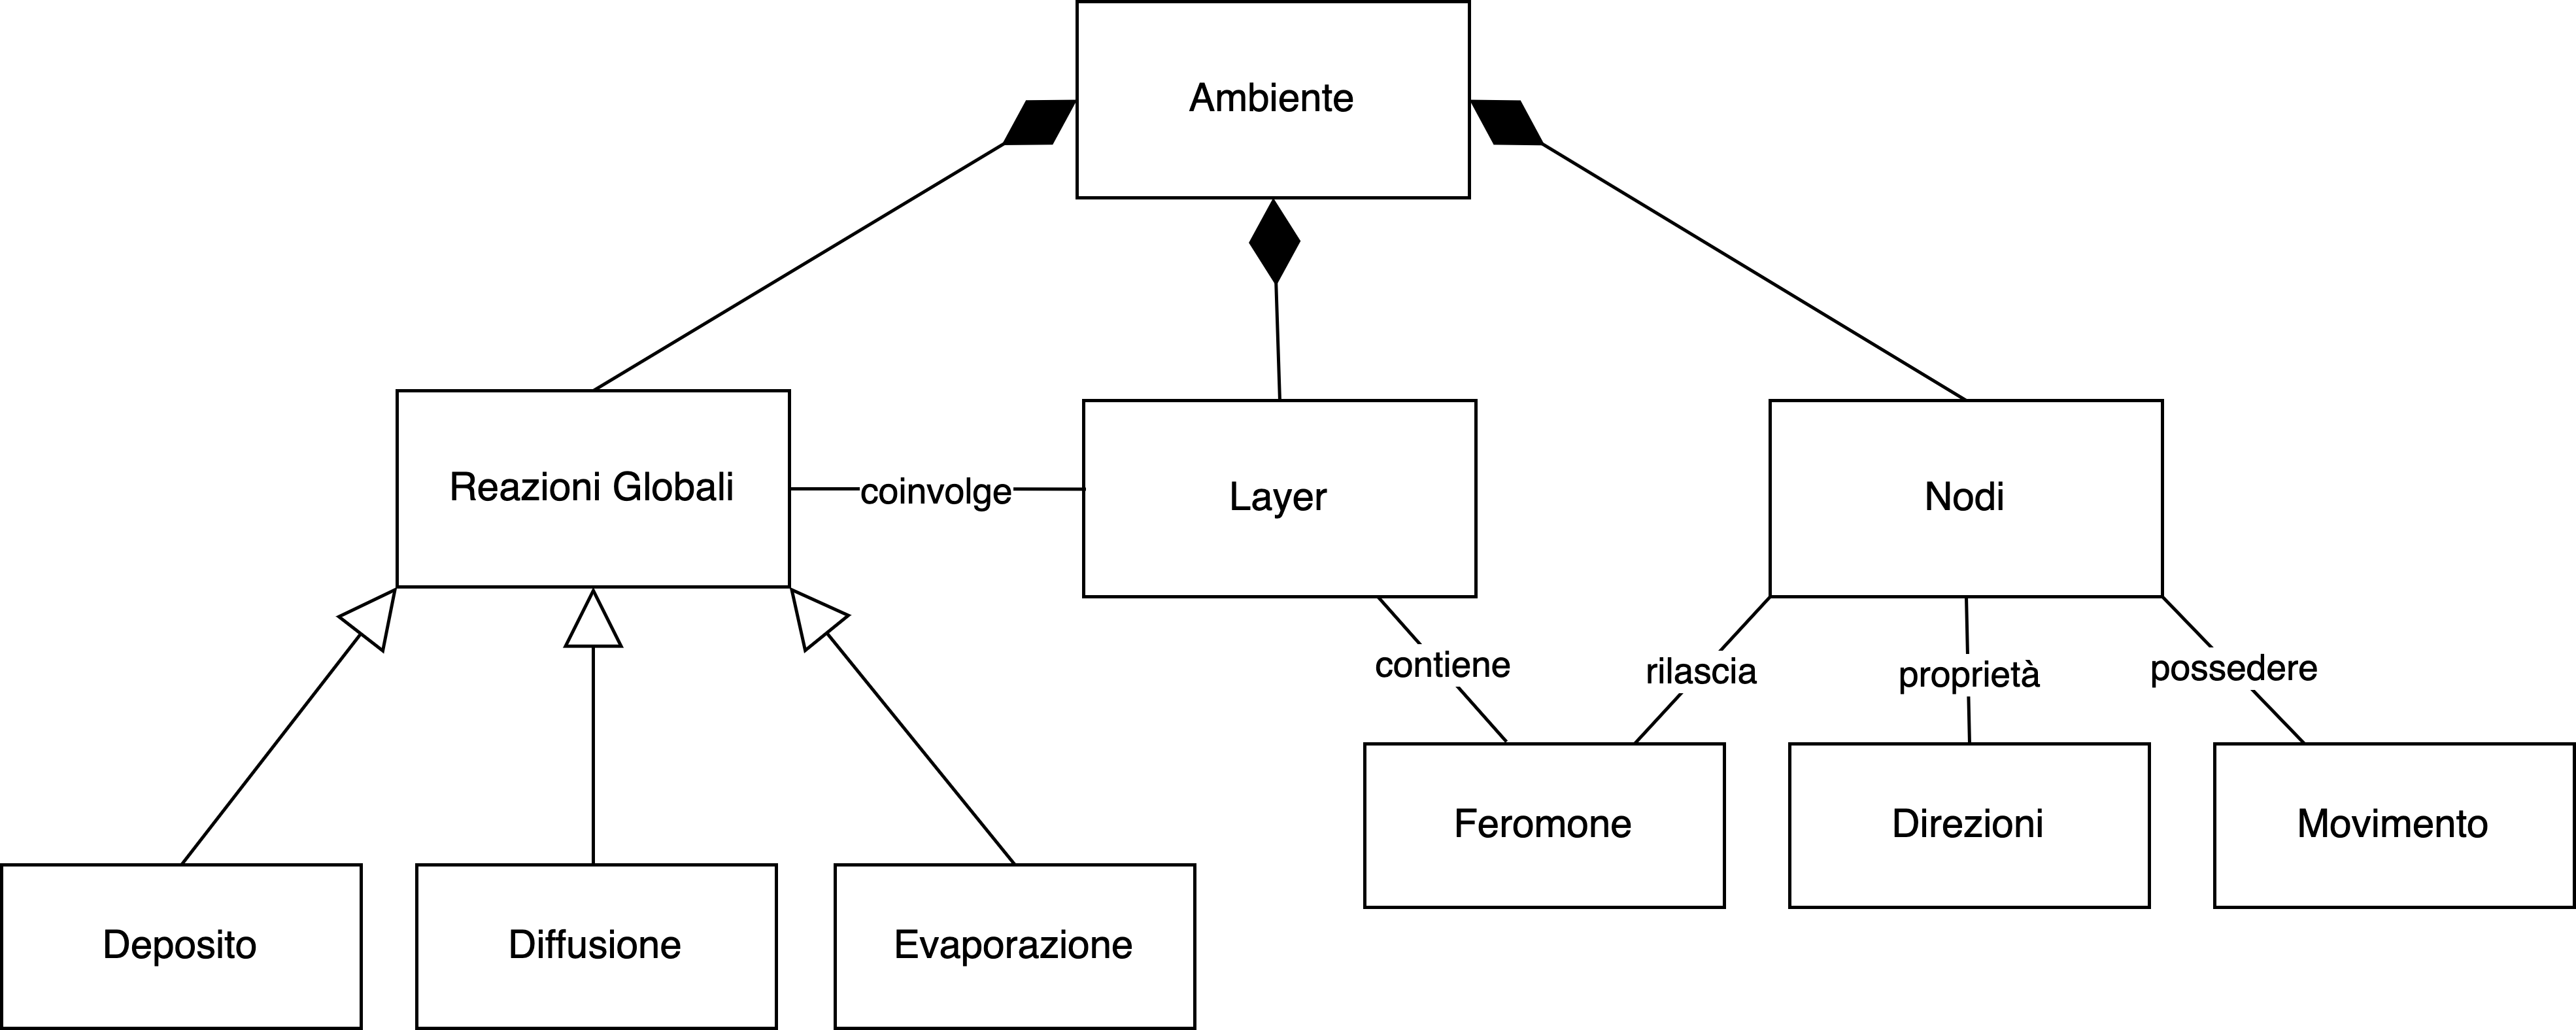
\includegraphics[width=0.9\textwidth]{figures/generale.png}
    \caption{Schema geneale del dominio.}\label{fig:generale}
\end{figure}\newline

Non sono stati individuati ulteriori requisiti specifici per la realizzazione di questo progetto di tesi.
Lo scopo di questa ricerca, infatti, è stato soprattutto quello di comprendere come il simulatore Alchemist 
potesse essere in grado di simulare questi comportamenti, tramite lo sviluppo un modello
dimostrativo.